\documentclass{article}
\usepackage[T1]{fontenc}
\usepackage{lmodern}
\usepackage{amssymb,latexsym,amsmath,stmaryrd,dk,dkenv}
\usepackage{tikz}
\usepgflibrary{shapes}
\usetikzlibrary{arrows,automata,backgrounds}
\usepackage{bbm}

\usepackage[all]{xy}
\usepackage{algorithm}
\usepackage[noend]{algpseudocode}

\DeclareFontFamily{U}{mathb}{\hyphenchar\font45}
\DeclareFontShape{U}{mathb}{m}{n}{<5> <6> <7> <8> <9> <10> gen * mathb <10.95> mathb10 <12> <14.4> <17.28> <20.74> <24.88> mathb12}{}
\DeclareSymbolFont{mathb}{U}{mathb}{m}{n}
\DeclareMathSymbol\fsmash\mathbin{mathb}{"0C}

\newcommand\den[1]{\llbracket #1\rrbracket}
\newcommand\rsem[1]{[#1]}
\newcommand\lsem[1]{L\den{#1}}
\newcommand\cset[1]{\{#1\}}
\newcommand\Rel{\kw{Rel}}
\newcommand\KL{\kw{Kl}}
\newcommand\KLP{\ensuremath{\KL\,\PP}} 
\newcommand\lam[2]{\lambda{#1}\kern1pt.\kern1pt{#2}}
\newcommand\nf[1]{#1^{\mathrm{nf}}}
\newcommand\CA{\ensuremath{P}}
\newcommand\At{\ensuremath{\mathit{At}}}
\newcommand\cseq[2]{\pseq{\pseq{#1}\cdots}{#2}}
\renewcommand\smash{\mathrel{\diamond}}
\newcommand\ssum{\mathop{\textstyle\sum}}
\newcommand\sbigcup{\mathop{\textstyle\bigcup}}
\newcommand\pdup{\mathop{\mathsf{dup}}}
\newcommand\One{\mathbf{1}}
\newcommand\Two{\mathbf{2}}
\newcommand\Exp{\mathsf{Exp}}
\newcommand\bval[1]{[#1]}
\renewcommand\star{^{\textstyle *}}
\newcommand\id{\mathsf{id}}
\newcommand\NetHKC[2]{\texttt{NetKATEquiv}(#1,#2)}
\newcommand\pair[2]{\langle #1,#2\rangle}
\renewcommand\powerset[1]{2^{#1}}
\newcommand\JI{\At\cdot(P\cdot\pdup)\star\cdot P}
\newcommand\setJI{2^{\At\cdot P\cdot(\pdup\cdot P)^{\scriptstyle *}}}
\newcommand\funJI{(2^{\At \cdot P})^{(P\cdot\pdup)^{\scriptstyle *}}}
\newcommand\acc{\mathsf{Accept}}
\newcommand\clname{\mathrm{cl}}
\newcommand\cl[1]{\clname(#1)}

\begin{document}

\begin{theorem}
$\den e = L(M_e)$.
\end{theorem}

\begin{definition}
{\em NetKAT$_{\text{DM}}$} is the subset of NetKAT such that De Morgan has
been applied to tests (predicates) so that all negations are applied only to
primitive tests.
\end{definition}

\begin{proof} Assume wlog that De Morgan has been applied to tests (predicates)
within $e$, so that $e \in$ NetKAT$_{\text{DM}}$. Proof by induction on 
following the recursive definition of NetKAT$_{\text{DM}}$.

\begin{description}

\item[Idea.] All expressions in NetKAT$_{\text{DM}}$ can be obtained from 
$f=n$, $f \neq n$, $f \gets n$ by using union ($+$), concatenation ($;$), and 
Kleene star ($\star$) operations. So it will suffice to show that:
\begin{itemize}
  \item $\den{f=n} = L(M_f=n)$
  \item $\den{f \neq n} = L(M_f \neq n)$
  \item $\den{f \gets n} = L(M_{f \gets n})$
  \item For any NetKAT$_{\textnormal{DM}}$ expressions $e_1$ and $e_2$: if
  $\den{e_1} = L(M_{e_1})$ and $\den{e_2} = L(M_{e_2})$, then 
  $\den{e_1+e_2} = L(M_{e_1+e_2})$, $\den{e_1;e_2} = L(M_{e_1;e_2})$, and
  $\den{e_1\star} = L(M_{e_1\star})$.
\end{itemize}
   
  
\item[Basis Step.]
\mbox{ }
  
\begin{itemize}
  \item $f=n$:
  \begin{figure}[H]
    \centering
    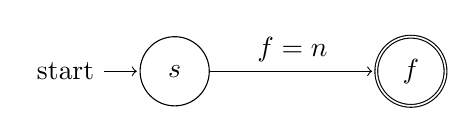
\begin{tikzpicture}[shorten >=1pt, auto]
      \node[state, initial]   (s)           {$s$};
      \node[state, accepting] (f) at (3,0)  {$f$};
  
      \path[->] (s) edge node {$f=n$} (f);
    \end{tikzpicture}
    \caption{$M_{f=n}$}
  \end{figure}
  
  From the denotational view of $L(M_e)(h)$,
  $L(M_{f=n})(pk::h) = \bigcup_{t\in F}\ell(t) = \ell(f)$. Since 
  $s \in S_{M_{f=n}}$, $\ell(s) = \{pk::h\}$. So, 
  $\ell(f) = \begin{cases} \{pk::h\}, & pk.f = n \\ \emptyset, 
  & otherwise \end{cases}$. So, $L(M_{f=n})(pk::h) = \den{f=n}(pk::h)$.


  \item $f \neq n$:
  \begin{figure}[H]
    \centering
    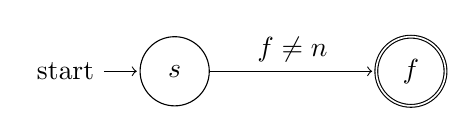
\begin{tikzpicture}[shorten >=1pt, auto]
      \node[state, initial]   (s)           {$s$};
      \node[state, accepting] (f) at (3,0)  {$f$};
  
      \path[->] (s) edge node {$f \neq n$} (f);
    \end{tikzpicture}
    \caption{$M_{f \neq n}$}
  \end{figure}
  
  From the denotational view of $L(M_e)(h)$,
  $L(M_{f \neq n})(pk::h) = \bigcup_{t\in F}\ell(t) = \ell(f)$. Since 
  $s \in S_{M_{f \neq n}}$, $\ell(s) = \{pk::h\}$. So, 
  $\ell(f) = \begin{cases} \{pk::h\}, & pk.f \neq n \\ \emptyset, 
  & otherwise \end{cases}$. Hence, 
  $L(M_{f \neq n})(pk::h) = \den{f \neq n}(pk::h)$.
  
  \item $f \gets n$:
  \begin{figure}[H]
    \centering
    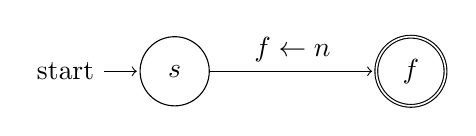
\begin{tikzpicture}[shorten >=1pt, auto]
      \node[state, initial]   (s)           {$s$};
      \node[state, accepting] (f) at (3,0)  {$f$};
  
      \path[->] (s) edge node {$f \gets n$} (f);
    \end{tikzpicture}
    \caption{$M_{f \gets n}$}
  \end{figure}
  
  From the denotational view of $L(M_e)(h)$,
  $L(M_{f \gets n})(pk::h) = \bigcup_{t\in F}\ell(t) = \ell(f)$. Since 
  $s \in S_{M_{f \gets n}}$, $\ell(s) = \{pk::h\}$. So, 
  $\ell(f) = \alpha\subst nf$. Hence, 
  $L(M_{f \gets n})(pk::h) = \den{f \gets n}(pk::h)$.
\end{itemize}
  
\item[Inductive Step.] For any NetKAT$_{\textnormal{DM}}$ expressions $p$ and 
$q$: if $\den{p} = L(M_{p})$ and $\den{q} = L(M_{q})$, then 
$\den{p+q} = L(M_{p+q})$, $\den{p;q} = L(M_{p;q})$, and
$\den{p\star} = L(M_{p\star})$.

\begin{itemize}
  \item $p+q$:
  \begin{figure}[H]
    \centering
    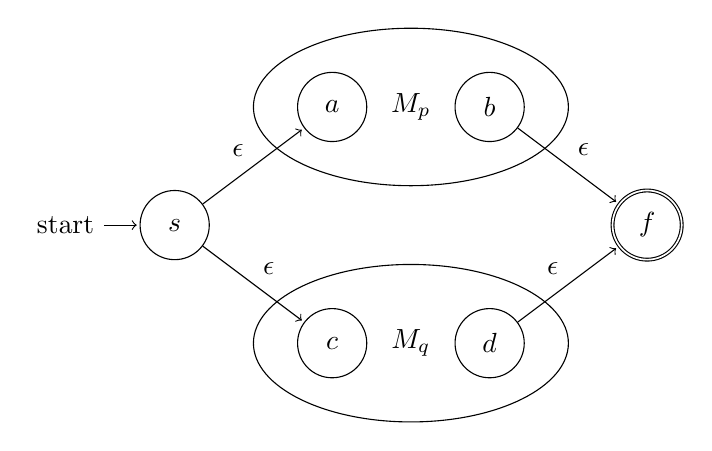
\begin{tikzpicture}[shorten >=1pt, auto]
      %\draw[help lines] (0,-3) grid (6,3);
      \draw (3,1.5) ellipse (2cm and 1cm) node {$M_p$};
      \draw (3,-1.5) ellipse (2cm and 1cm) node {$M_q$};
  
      \node[state, initial]   (s)             {$s$};
      \node[state]            (a) at (2,1.5)  {$a$};
      \node[state]            (b) at (4,1.5)  {$b$};
      \node[state]            (c) at (2,-1.5) {$c$};
      \node[state]            (d) at (4,-1.5) {$d$};
      \node[state, accepting] (f) at (6,0)    {$f$};
  
      \path[->] (s) edge node {$\epsilon$} (a)
                    edge node {$\epsilon$} (c)
                (b) edge node {$\epsilon$} (f)
                (d) edge node {$\epsilon$} (f);
    \end{tikzpicture}
    \caption{$M_{p+q}$}
  \end{figure}
  
  From the denotational view of $L(M_e)(h)$,
  $L(M_{p+q})(h) = \bigcup_{t\in F}\ell(t) = \ell(f)$. Since 
  $s \in S_{M_{p+q}}$, $\ell(s) = \ell(a) = \ell(c) = \{h\}$. Since 
  $a \in S_{M_p}$ and $b \in F_{M_p}$, $\ell(b) = L(M_p)(h)$. Since 
  $c \in S_{M_q}$ and $d \in F_{M_q}$, $\ell(d) = L(M_q)(h)$. So, 
  $L(M_e)(h) = L(M_p)(h) \cup L(M_q)(h)$. Thus, by the inductive hypothesis,
  $L(M_p+q)(h) = \den{p+q}(h)$. 
  
  \item $p;q$:
  \begin{figure}[H]
    \centering
    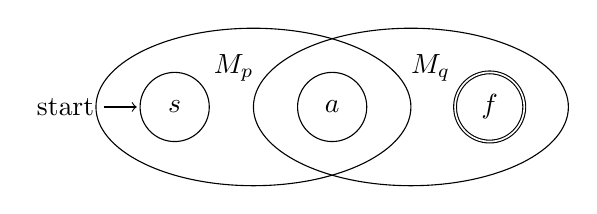
\begin{tikzpicture}[shorten >=1pt, auto]
      %\draw[help lines] (0,-3) grid (6,3);
      \draw (1,0) ellipse (2cm and 1cm);
      \draw (.75,.5) node {$M_p$};
      \draw (3,0) ellipse (2cm and 1cm);
      \draw (3.25,.5) node {$M_q$};
  
      \node[state, initial]   (s)           {$s$};
      \node[state]            (a) at (2,0)  {$a$};
      \node[state, accepting] (f) at (4,0)  {$f$};
    \end{tikzpicture}
    \caption{$M_{p;q}$}
  \end{figure}
  
  From the denotational view of $L(M_e)(h)$,
  $L(M_{p+q})(h) = \bigcup_{t\in F}\ell(t) = \ell(f)$. Since 
  $s \in S_{M_{p;q}}$, $\ell(s) = \{h\}$. Since $a \in F_{M_p}$, 
  $\ell(a) = L(M_p)(h)$. Since $a \in S_{M_q}$ and $f \in F_{M_q}$,
  $\ell(f) = (L(M_p) \cdot L(M_q))(h)$. Thus, by the inductive hypothesis, 
  $L(M_{p;q})(h) = \den{p;q}(h)$.
  
  \item $p\star$:
  \begin{figure}[H]
    \centering
    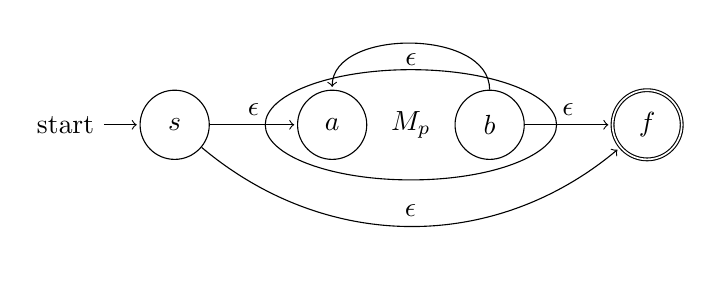
\begin{tikzpicture}[shorten >=1pt, auto]
      %\draw[help lines] (0,-3) grid (6,3);
      \draw (3,0) ellipse (1.85cm and .7cm) node {$M_p$};
  
      \node[state, initial]   (s)           {$s$};
      \node[state]            (a) at (2,0)  {$a$};
      \node[state]            (b) at (4,0)  {$b$};
      \node[state, accepting] (f) at (6,0)  {$f$};
  
      \path[->] (s) edge                 node {$\epsilon$} (a)
                    edge [bend right=40] node {$\epsilon$} (f)
                (b) edge [bend right=90] node {$\epsilon$} (a)
                    edge                 node {$\epsilon$} (f);
    \end{tikzpicture}
    \caption{$M_{p\star}$}
  \end{figure}
  
  From the denotational view of $L(M_e)(h)$,
  $L(M_{p\star})(h) = \bigcup_{t\in F}\ell(t) = \ell(f)$. Since 
  $s \in S_{M_{p\star}}$, $\ell(s) = \{h\}$. Since $a \in S_{M_p}$, 
  $\ell(a) = \ell(s) \cup \ell(b)$, and $b \in F_{M_p}$,
  $\ell(b) = \bigcup_{i \in \mathbb{N} \backslash \{0\}} G^i(h)$, where 
  $G^{1}(h) = L(M_p)(h)$ and $G^{i+1}(h) = (L(M_p) \cdot G^i)(h)$ . So,
  $\ell(f) = {h} + \ell(b) = \bigcup_{i \in \mathbb{N}} F^i(h)$, where 
  $F^{0}(h) = {h}$ and $F^{i+1} = (L(M_p) \cdot F^i)(h)$. Thus, by the
  inductive hypothesis, $L(M_{p\star}(h) = \den{p\star}(h)$.
\end{itemize}
\end{description}
\end{proof}

\end{document}
